\chapter{\textsc{Analyse du procédé de deux bacs d'eau avec régulation}}
\section{\textsc{Le procédé}}
	
	\paragraph{} Le système représenté sur la Figure 3 est composé de deux bacs cylindriques de section $S$. Ils sont reliés par un tuyau d’écoulement de section $S_n << S$. Le dernier bac se vide par un cylindre (également de section $S_n$ )
dans un réservoir situé sous les bacs. Une pompe de débit $Q(t) = K_debit u(t)$ permet de remplir respectivement
les bacs avec l’eau récupérée dans le réservoir. Le système fonctionne en circuit fermé. La pompe est alimentée
par une tension, $u$, et la relation entre la loi de commande et le débit est donnée par le paramètre $K_debit$ . Lors
de cette manipulation, nous allons nous intéresser à la régulation de niveau de l’eau $H_1 (t)$ et $H_2 (t)$.

\paragraph{} Les valeurs données par le constructeur sont : $K_debit = 1.4 \times 10^{-4} m^2/sV , Q_0 = 12 \times 10^{-5} m^3/s, S = 0.0154m^2$ et $S_n = 5 \times 10^{-5} m^2$. Les valeurs initiales sont $H_1(0) = 0.3m$ et $H_2(0) = 0.2m$.
On suppose que les vitesses de $H_1 (t)$ et $H_2 (t), v_1 (t), v_2 (t)$ respectivement, sont plus petites que la vitesse du fluide qui circule par les tuyaux de section $S_n , v_n (t),$ c.à.d. $v_1 (t) << v_{n1} (t)$ et $v_2 (t) << v_{n2} (t)$.

	\begin{center}
	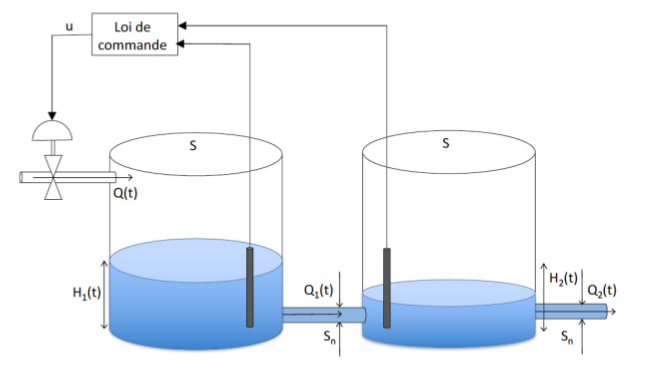
\includegraphics[scale=0.5]{3bac.png}
	\captionof{figure}{\textit{Deux bacs d'eau avec source et fuite\\}}
	\label{fig3} 
	\end{center} 

\section{\textsc{Modélisation du système par un bilan de volume}}

	Nous avons:
\begin{center}

   $ V_1(t)=S\times (H_1(t)-H_2(t))$\\[0.5cm]   
    
  $\dot{V}_1(t)= S \times (\dot{H}_1(t)-\dot{H}_2(t))=(Q(t)-Q_1(t)); \hspace{2mm} Q(t) = S_n \frac{\sqrt{2gH_2}} {K_{debit}}.\\[0.5cm]
  
    Q_1(t)=S_n \times v_{n_1} \hspace{3mm}$ avec:$\hspace{1mm}  v^2_{n_1} = 2 \times g\times |H_1(t)-H_2(t)| \\[1 cm]$
 
 Et:
    $V_2(t)=S\times H_2(t)$\\[0.5cm]

   $ \dot{V}_2(t) = S \times \dot{H}_2(t)=(Q_1(t)-Q_2(t)); \hspace{2mm} Q_1(t):$ à trouver\\[0.5cm]
    
    $Q_2(t) = S_n \times v_{n_2} \ ; \hspace{3mm}$ avec:$\hspace{1mm}  v^2_{n_2} = 2 \times g \times H_2(t)    \\[1 cm]$
\end{center} 


Donc $Q_1(t)=S_n\sqrt{2g |H_1(t)-H_2(t)|}$ et $ Q_2(t)=S_n\sqrt{2gH_2(t)} $\\
\par On pose:  $ x_1 = (H_1(t) - H_2(t)) > 0 \hspace{2mm} \forall t$ et $ x_2 = H_2(t) $.\\

\[\Longrightarrow Q_1=S_n\times \sqrt{2\times g \times x_1}\]
\[\Longrightarrow Q=S_n\times \frac{\sqrt{2\times g \times x_2}}{K_{debit}} \]
\[\Longrightarrow \dot{x}_1=\frac{Q}{S}-\frac{Q_1}{S}= \frac{S_n\times \sqrt{2\times g }}{S \times K_{debit} } \times \sqrt{x_2} - \frac{S_n\times \sqrt{2\times g }}{S} \times \sqrt{x_1} \] \\[0.5 cm]

\[\Longrightarrow Q_2=S_n\times \sqrt{2\times g \times x_2}\]
\[\Longrightarrow \dot{x}_2=\frac{Q_1}{S}-\frac{Q_2}{S}= \frac{S_n\times \sqrt{2\times g }}{S} \times \sqrt{x_1} - \frac{S_n\times \sqrt{2\times g }}{S} \times \sqrt{x_2} \]
 

\section{\textsc{Détermination des points d'équilibres}}
 
	\par 


